% !TeX root=../main.tex

\chapter{پاسخ سوالات سری اول}

% دستور زیر باعث عدم‌نمایش شماره صفحه در اولین صفحهٔ این فصل می‌شود.
%\thispagestyle{empty}
\section{ پاسخ سوال 1}

\subsection{بخش 1}

\subsubsection{قسمت یک}
برای حل این مسئله ی بهینه سازی، با استفاده از یک کد متلب ابتدا نابرابری های داده شده در یک نمودار دو بعدی ترسیم شده و ناحیه ی اشتراک حاصل از این خطوط  برای پاسخ های ممکن به دست می آید.



\begin{figure}
	\centering
	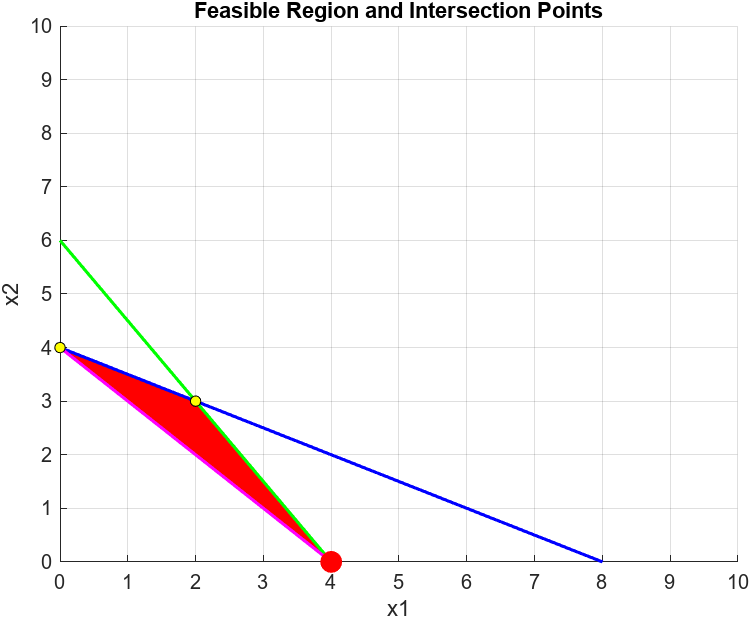
\includegraphics[width=1\linewidth]{../img/Q1_1}
	\caption{}
	\label{fig:q11}
\end{figure}

پاسخ بهینه برای معادله ی 
	\( f(x_1, x_2) = 5x_1 + 6x_2 \)
با جایگذاری مقادیر ممکن در معادله به دست می آید.
	
	\begin{itemize}
		\item \( (x_1 = 2.00, x_2 = 3.00) \), \( f(x_1, x_2) = 28.00 \)
		\item \( (x_1 = 0.00, x_2 = 4.00) \), \( f(x_1, x_2) = 24.00 \)
		\item \( (x_1 = 4.00, x_2 = 0.00) \), \( f(x_1, x_2) = 20.00 \)
		\item \( (x_1 = 0.00, x_2 = 4.00) \), \( f(x_1, x_2) = 24.00 \)
		\item \( (x_1 = 4.00, x_2 = 0.00) \), \( f(x_1, x_2) = 20.00 \)
	\end{itemize}
	
جواب بهینه برای این سوال برابر خواهد بود با:
	\[
	(x_1 = 4.00, x_2 = 0.00) , \quad f(x_1, x_2) = 20.00
	\]
\subsubsection{قسمت دو}
در این مرحله، با استفاده از ابزار های 
Yalmip
, 
CVX
مسئله ی بهینه سازی را حل می کنیم. در بخش اول، با استفاده از کد متلب زیر، محدودیت ها و تابع هزینه تعریف شده و در نهایت با اجرای کد، جواب های مورد نظر به دست می آید.


با استفاده از این کد، در نهایت جواب هایی مطابق با آنچه که به روش تحلیلی به دست آمد، حاصل می شود.

\[
(x_1 = 4.00, x_2 = 0.00) , \quad f(x_1, x_2) = 20.00
\]
در گام بعد، با استفاده از پکیج های CVX و fmincon، بار دیگر این مسئله حل می شود.



\[
(x_1 = 4.00, x_2 = 0) , \quad f(x_1, x_2) = 20.00
\]

مشاهده می شود که با استفاده از این روش نیز، پاسخ مشابهی به دست می آید.

\subsection{بخش 2}
در این بخش، مشابه آنچه که در بخش پیشین انجام شد، ابتدا به روش تحلیلی و با رسم ناحیه ی نقاط امکان پذیری، نقاط بهینه تشخیص داده می شوند.
در کد متلب زیر، با تعیین معادلات مربوط به محدودیت ها، و محاسبه ی نقاط تقاطع خطوط، پاسخ بهینه به دست آمده و نمایش داده شده است.




\begin{figure}[H]
	\centering
	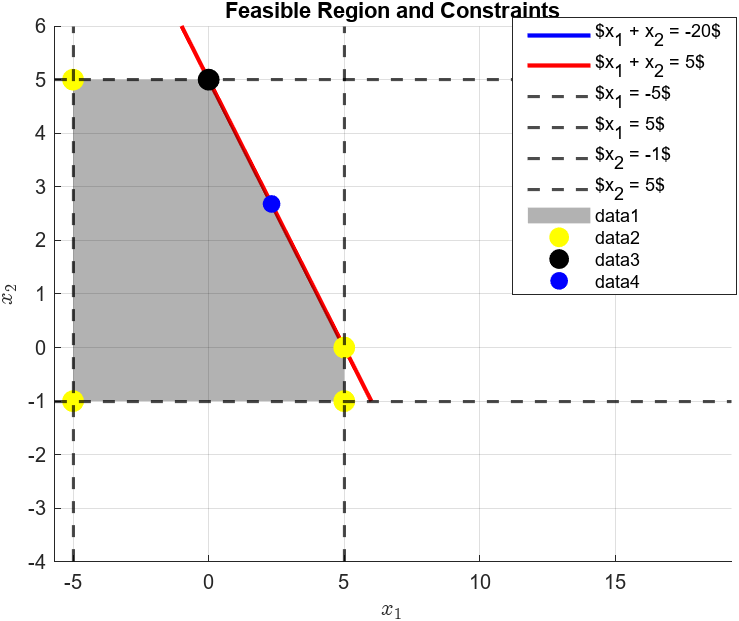
\includegraphics[width=1\linewidth]{../img/Q2_11}
	\caption{}
	\label{fig:q21}
\end{figure}

	
پاسخ بهینه برای تابع هزینه، با جایگذاری نقاط در آن و انتخاب مقدار کمینه به دست می آید.

\[
(x_1 = 0.00, x_2 = 5) , \quad f(x_1, x_2) = 5
\]

در قسمت بعد، بار اول با استفاده از پکیج 
Yalmip
و بار دیگر با استفاده از پکیج 
CVX
مسئله ی بهینه سازی را حل می کنیم.

\textbf{Yalmip:}


\[
(x_1 = 5.00, x_2 = 0) , \quad f(x_1, x_2) = 5.00
\]

CVX:

\[
(x_1 = 2.32, x_2 = 2.68) , \quad f(x_1, x_2) = 5.00
\]

fmincon:
\[
(x_1 = 2.4637, x_2 = 5363) , \quad f(x_1, x_2) = 5.00
\]
مشاهده می شود که پاسخ به دست آمده توسط روش این روش ها با یکدیگر تفاوت دارد. در حالی که جواب CVX و fmincon از نقاط گوشه نیست، اما پاسخ درستی برای مسئله ی بهینه سازی است و می تواند به عنوان نقطه ی بهینه انتخاب شود.



\section{پاسخ سوال 2}
در این سوال، مانند قسمت قبل باید ابتدا تابع هزینه و سپس محدودیت ها مشخص شوند. تفاوت این سوال، به دلیل تغییر در نحوه ی بیان محدودیت ها است که در غالب ماتریس داده شده است. بنابراین، با تبدیل آن به فرم معادلات خطی خواهیم داشت:

\begin{align*}
	x_1 - 2x_2 &\geq -2, \\
	-x_1 - 2x_2 &\geq -6, \\
	-x_1 + x_2 &\geq -2, \\
	x_1 &\geq 0, \\
	x_2 &\geq 0.
\end{align*}

برای حل این سوال و استفاده از پکیج های یاد شده
  در کدهای متلب که در ادامه آمده است، مسئله ی بهینه سازی را حل می کنیم.

\textbf{Yalmip:}


\[
(x_1 = 1.4, x_2 = 1.7) , \quad f(x_1, x_2) = 0.8
\]

\textbf{CVX:}



\[
(x_1 = 1.4, x_2 = 1.7) , \quad f(x_1, x_2) = 0.8
\]

\textbf{fmincon:}
\[
(x_1 = 1.4, x_2 = 1.7) , \quad f(x_1, x_2) = 0.8
\]


مشاهده می شود که با استفاده از هر دو روش، نتایج یکسانی به دست می آید.

\section{پاسخ سوال 3}

با توجه به معادله ی داده شده در این سوال، مشاهده می شود که بر خلاف مسائل پیشین، در این مثال نواحی مرزی تعیین نشده است و یک مثال بهینه سازی نامحدود است. پیش از انجام محاسبات به روش تحلیلی و پیدا کردن نقطه ی کمینه، ابتدا با رسم نمودار معادله، درکی از رفتار آن به دست می آوریم.



\begin{figure}[H]
	\centering
	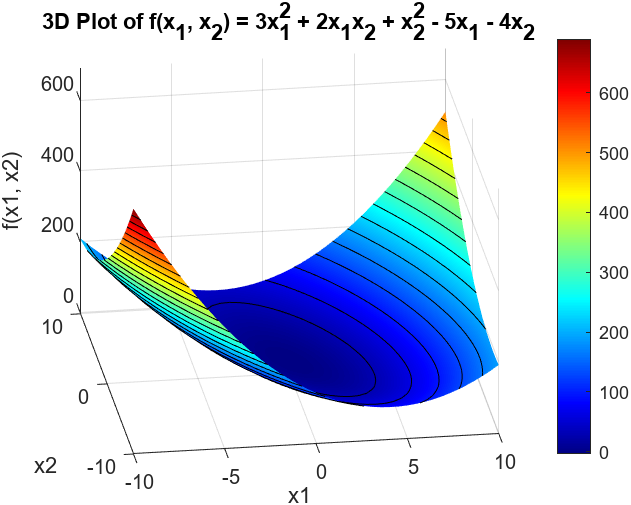
\includegraphics[width=1\linewidth]{../img/Q3_1}
	\caption{}
	\label{fig:q31}
\end{figure}

همان طور که بیان شد، مشاهده می شود که می توان یک نقطه ی کمینه برای این مثال پیدا کرد.

با در اختیار داشتن معادله که در این قسمت مجددا آورده شده است، لازم است مشتق آن نسبت به x1 و x2 گرفته شده و با برابر صفر قرار دادن هر یک از آنها، مقادیر مورد نظر به دست آید. در ادامه ی این بخش، به شرح این فرایند خواهیم پرداخت.

\[
f(x_1, x_2) = 3x_1^2 + 2x_1x_2 + x_2^2 - 5x_1 - 4x_2
\]


مشتق اول عبارت فوق برابر است با:

\[
\nabla f(x_1, x_2) = \left[ \frac{\partial f}{\partial x_1}, \frac{\partial f}{\partial x_2} \right] = \left[ 6x_1 + 2x_2 - 5, 2x_1 + 2x_2 - 4 \right]
\]

با برابر صفر قرار دادن مشتقات خواهیم داشت:

\[
6x_1 + 2x_2 - 5 = 0
\]
\[
2x_1 + 2x_2 - 4 = 0
\]


از حل این معادله، به دست می آید:

\[
x_1 = \frac{1}{4}, \quad
x_2 = \frac{7}{4}
\]

با محاسبه ی ماتریس مشتق مرتبه دوم و بررسی المان های ماتریس هسین، می توانیم مشخص کنیم که نقاط به دست آمده، از چه نوع اکسترمم هستند. برای این کار خواهیم داشت:

\[
H = \begin{bmatrix}
	\frac{\partial^2 f}{\partial x_1^2} & \frac{\partial^2 f}{\partial x_1 \partial x_2} \\
	\frac{\partial^2 f}{\partial x_2 \partial x_1} & \frac{\partial^2 f}{\partial x_2^2}
\end{bmatrix} = \begin{bmatrix}
	6 & 2 \\
	2 & 2
\end{bmatrix}
\]

از آنجا که ماتریس هسین به دست آمده مثبت معین است، بنابراین نقاط به دست آمده، معادل نقطه ی مینیمم می باشند.

در مرحله ی بعد، با استفاده از پکیج های بهینه سازی، به حل این مسئله خواهیم پرداخت.

\textbf{Yalmip:}


\[
(x_1 = 0.25, x_2 = 1.75) , \quad f(x_1, x_2) = -4.1250
\]

\textbf{fmincon:}
\[
(x_1 = 0.25, x_2 = 1.75) , \quad f(x_1, x_2) = -4.1250
\]
\textbf{CVX:}


با اجرای کد CVX، مشاهده می شود که این پکیج قادر به حل این مسئله نیست و با خطا روبه رو می شود. دلیل این مسئله آن است که تابع داده شده محدب نیست و در نقطه ای مشتق ان برابر صفر می شود و پکیج 
CVX 
قادر به حل مسائل غیرمحدب نیست.

در بخش بعد، برای پیدا کردن نقطه ی ماکسیمم، باید علامت منفی در تابع ضرب شود. بنابراین، مطاب قآنچه که در نمودار نمایش داده شده برای این معادله دیده شد و همچنین با توجه به ماهیت معادله که محدب و نامحدود است، می توان نتیجه گرفت که این معادله مقدار بیشینه ای ندارد و یا مقدار آن برابر بی نهایت است. 
در محاسبه ی تحلیلی این قضیه، مشاهده کردیم که تنها یک جواب به دست آمد و با بررسی ماتریس هسین دیدیم که این مقدار، مربوط به مینیمم تابع است. بنابراین، به روش تحلیلی می توان نتیجه گرفت که این معادله مقدار ماکسیمم ندارد.

در ادامه با استفاده از پکیج های Yalmip و CVX، صحت این موضوع را بررسی می کنیم.

\textbf{Yalmip:}


\[
(x_1 = -243236479749.1021, x_2 = -130439567620.7782) 
\]

\[
\quad f(x_1, x_2) = 257961758541185663631360.0000
\]

مشاهده می شود که مقادیر گزارش شده به دلیل محدودیت در انجام محاسبات است و بیشتری

\textbf{CVX:}


مجددا مشاهده می شود که CVX نمی تواند این مسئله را حل کند.

\section{پاسخ سوال 4}
 
 برای حل این سوال، با بررسی تابع داده شده در می یابیم که به دلیل وجود ریشه چهارم در این عبارت، مقعر است. بنابراین، می توانیم اطمینان داشته باشیم که استفاده از پکیج های Yalmip و CVX قادر به حل این مسئله نخواهند بود.
 % TODO: \usepackage{graphicx} required
 \begin{figure}[H]
 	\centering
 	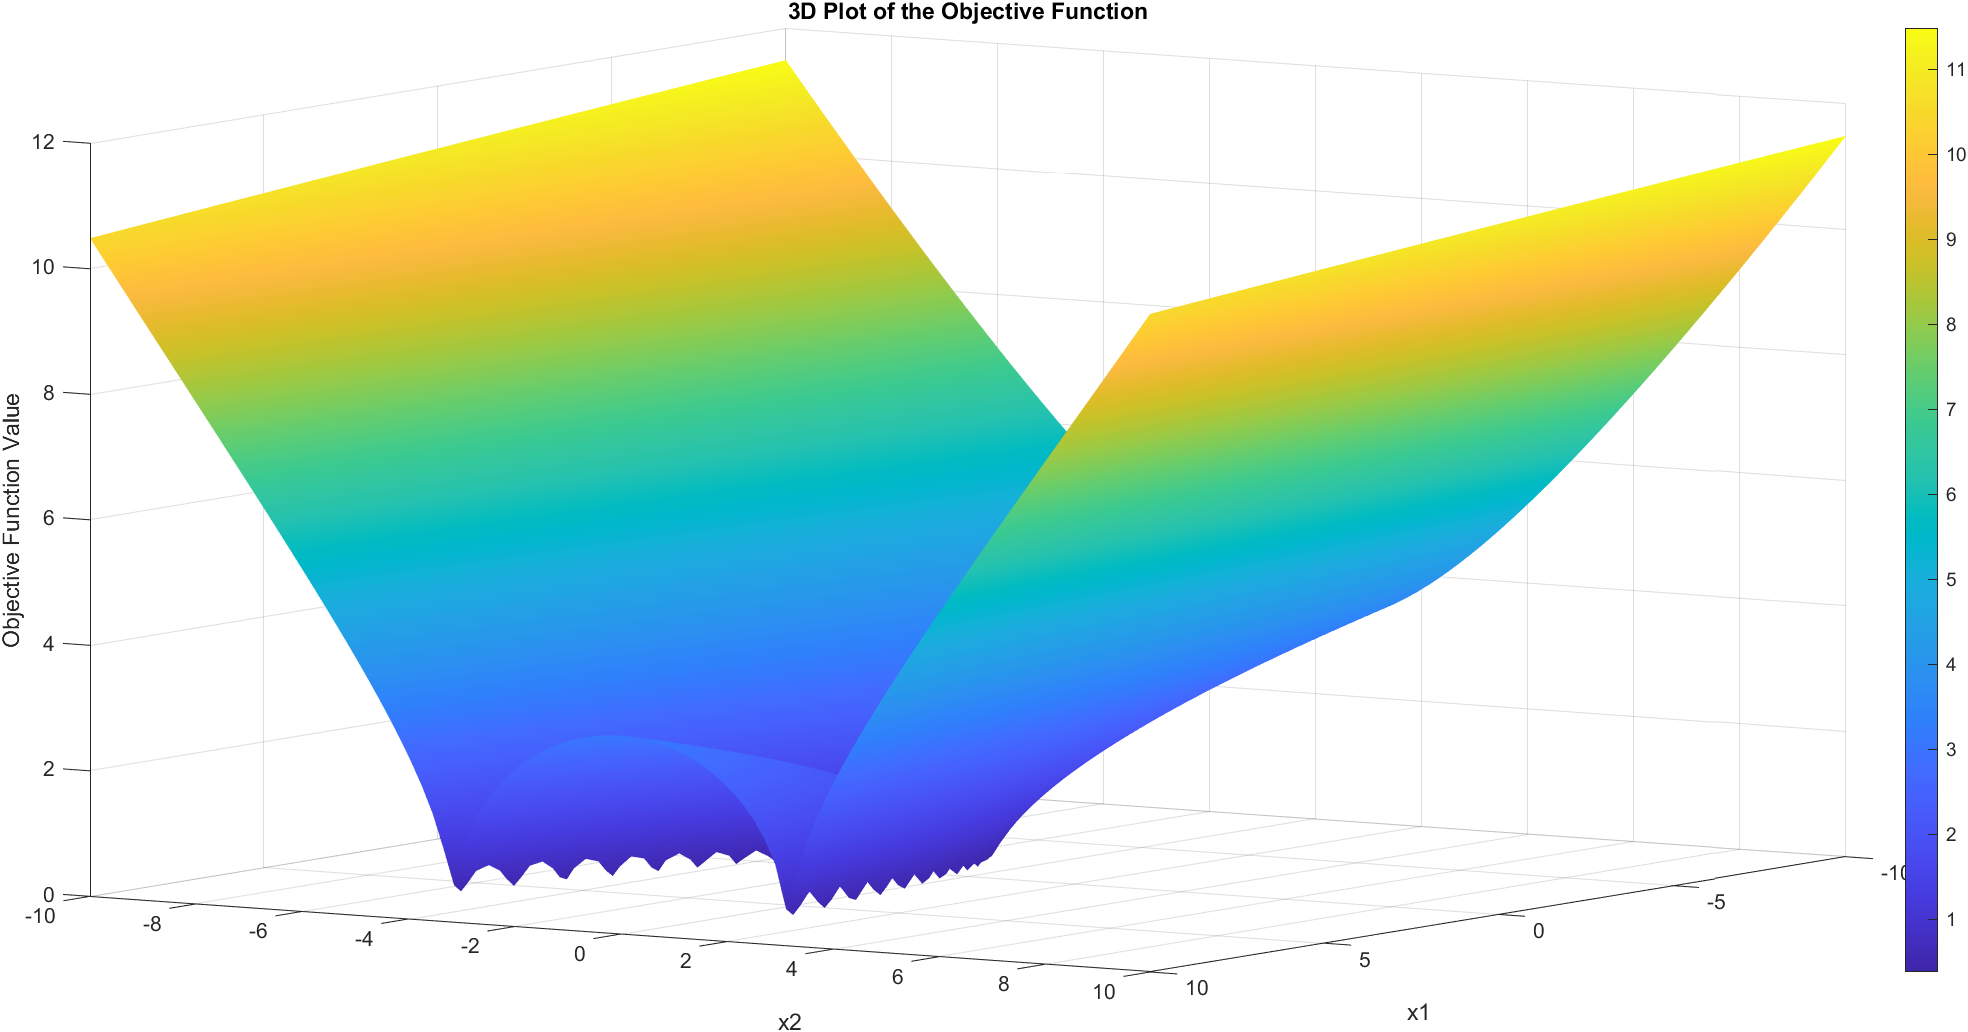
\includegraphics[width=1\linewidth]{../img/Q4}
 	\caption{}
 	\label{fig:q4}
 \end{figure}
  در ادامه، به اجرا و بررسی عملکرد این شبکه ها خواهیم پرداخت.
 
با اجرای کد متلب بهینه سازی برای این تابع مطابق آنچه که انتظار داشتیم، هیچ یک از این دو روش نتایجی به دست نمی دهد. علت این مشکل در گام اول محدب نبودن تابع داده شده است که به طور مشخص در فرایند پردازش الگوریتم 
CVX
اختلال ایجاد می کند. اما علت دوم، می تواند شکل گیری حالت گوشه در تابع در حالتی باشد که 

\[
x_1 \approx x_2^2
\]

در این حالت، معادله به طور نسبی مشتق پذیر نیست و به دلیل ععملکرد این دو الگوریتم بر اساس گرادیان کاهشی، نمیتوانند نتیجه را پیش بینی کنند.

بنابراین، با استفاده از الگوریتم های پیشرفته تر نظیر الگوریتم ژنتیک، تابع را بهینه سازی می کنیم.
 


   \textbf{GA:}

 \[
 (x_1 = 0.3987, x_2 = 0.6315) , \quad f(x_1, x_2) = 0.3800
 \]
 
 
 \section{پاسخ سوال 5}
روش 
 Cross Entropy
 یکی از روش های نوین بهینه سازی است که با ترکیب دانش آمار و احتمال و تکنیک های یادگیری ماشین، 
 سعی در بهینه سازی توابع داده شده می کند. در این روش که شباهتی نیز به الگوریتم ژنتیک دارد، ابتدا مجموعه ای از نقاط به صورت تصادفی انتخاب می شوند. سپس با جای گذاری این نقاط در تابع هدف، مقادیر متناظر هر یک انتخاب می شوند و سپس، با تعداد مشخصی از نقاط که پایخ های مناسب تری داشتند به عنوان نقاط برتر انتخاب می شوند. در گام بعد، با استفاده از این نقاط، توزیع احتمالی جدیدی حول این نقاط برتر شکل می گیرد و بار دیگر این فرایند انجام می شود. با تکرار این فرایند به تعداد مناسب و یا با برقرار شدن شرایط توقف، الگوریتم متوقف شده و بهترین پاسخ ارائه می شود.
 در این قسمت، با استفاده از این روش، سعی بر آن داریم تا معادله ی 
 \[
 f(x) = 10 \times 2 + \left( x_1^2 - 10 \cos(2 \pi x_1) \right) + \left( x_2^2 - 10 \cos(2 \pi x_2) \right) + \mathcal{N}(0, 0.1)
 \]
 را بهینه سازی کنیم. این تابع که با نام 
 Rastrigin
 شناخته می شود یکی از توابع پرکاربرد برای تست الگوریتم های بهینه سازی است. علت کاربرد زیاد این تابع آن است که این تابع دارای تعداد زیادی نقطه ی کمینه ی محلی است و همچنین مقعر است. بنابرین، معیار مناسبی برای بررسی عملکرد الگوریتم های بهینه سازی است.
 در تابع مورد استفاده در این بخشف از یک المان تصائفی نیز برای شبیه سازی نویز محیطی در سیگنال استفاده شده است.
 جهت درک بهتر این تابع، نمودار سه بعدی آن رسم شده است.
 


\begin{figure}[H]
	\centering
	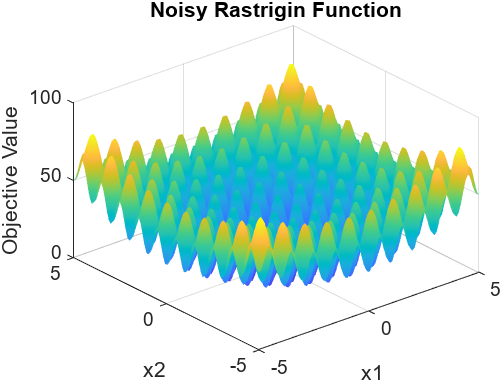
\includegraphics[width=1\linewidth]{../img/Rastrigin}
	\caption{}
	\label{fig:rastrigin}
\end{figure}

در کد نوشته شده برای این بخش، ابتدا پارامتر های اولیه شامل میانگین و واریانس اولیه، تعداد تکرار فرایند و تعداد انتخاب های برتر در هر تکرار مشخص می شود.
در ادامه، مطابق آنچه که گفته شد، در هر مرحله تعداد 100 نمونه به طور اتفاقی و با استفاده از میانگین و واریانس داده شده انتخاب می شوند و پس از جایگذاری مقادیر این نقاط در تابع و مرتب کردن مقادیر تابع، 10 نمونه که نتایج بهتری داشتند انتخاب می شوند. 
با تکرار این فرایند، در نهایت نقطه ی بهینه به صورت زیر به دست می آید.


\begin{figure}[H]
	\centering
	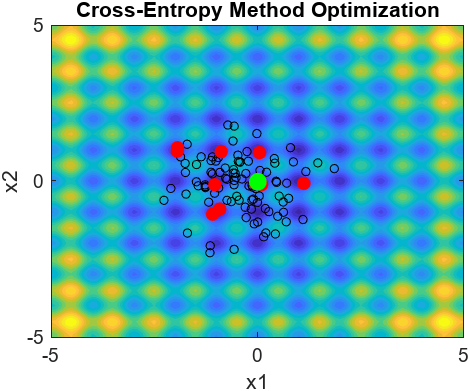
\includegraphics[width=1\linewidth]{../img/Q5}
	\caption{}
	\label{fig:q5}
\end{figure}
 
 \[
 (x_1 = 0.0081, x_2 = -0.0231) , \quad f(x_1, x_2) = 0.1060
 \]
 
 با مشاهده ی انیمیشن قرار داده شده در فایل متلب این تمرین، فرایند تشخیص پایخ بهینه نمایش داده شده است.
 
 
 
 
 